\section{Numerical Example}
\label{sec:numerical}
%

A Julia implementation of this algorithm may be found
in~\cite{satici_implementation}. The implementation allows the user to specify
how many data points to randomly generate and how many components to use in the
Gaussian mixture model. Once these are specified, the model can be trained by 
executing the \texttt{execute\_em!} function. 

The trained model with $N=1001$ sample points and $M=61$ components over the
range $-\pi \leq \theta_1, \theta_2, \theta_3 \leq \pi$ may be tested by running
the \texttt{test\_training} function, which generates $200$ extra points and
returns the average error incurred by the output of the algorithm. A
visualization of the performance of the algorithm is depicted in
Figure~\ref{fig:example_sol}. Table~\ref{tab:perf_wrt_components} compares how
the performance of the algoritm changes as the number of components $M$ is
varied for $N=2001$.
%
The posterior $P(\theta \mid \mathrm{x})$ is initialized with a uniform
covariance matrix with a mean coming from the initial $k$-means algorithm. As
the EM algorithm proceeds, our belief on $P(\theta \mid \mathrm{x})$ is updated.
The evolution of our belief is depicted in Figure~\ref{fig:belief_evolution}.

\begin{table}[t]
    \centering
    {\renewcommand{\arraystretch}{1.2}
\begin{tabular}{l|ccccccccc}
    Components & $41$ & $51$ & $61$ & $71$ & $81$ & $91$ & $101$ & $111$ & $121$ \\ \hline
    Mean $\ell_2$ error & $0.2368$ & $0.2104$ & $0.1613$ & $0.1795$ & $0.1685$ & 
    $0.1926$ & \fbox{$0.1392$} & $0.1792$ & $0.1584$
\end{tabular}
    }
\caption{The performance of the algorithm for different number of Gaussian 
components for $N = 2001$ data points, tested over $200$ fresh samples.}
\label{tab:perf_wrt_components}
\end{table}


% \begin{table}[b]
%     \centering
%     {\renewcommand{\arraystretch}{1.2}
% \begin{tabular}{l|cccccccc}
%     Components & $131$ & $141$ & $151$ & $161$ & $171$ & $181$ & $191$ & $201$  \\ \hline
%     Mean $\ell_2$ error & $0.1479$ & $0.1265$ & $0.1536$ & $0.1317$ & $0.1389$ & 
%     $0.1696$ & $0.1770$ & $0.1271$ 
% \end{tabular}
%     }
% \caption{Just for giggles: continuation of Table~\ref{tab:perf_wrt_components}.}
% % \label{tab:perf_wrt_components}
% \end{table}


\begin{figure}[t]
    \centering
	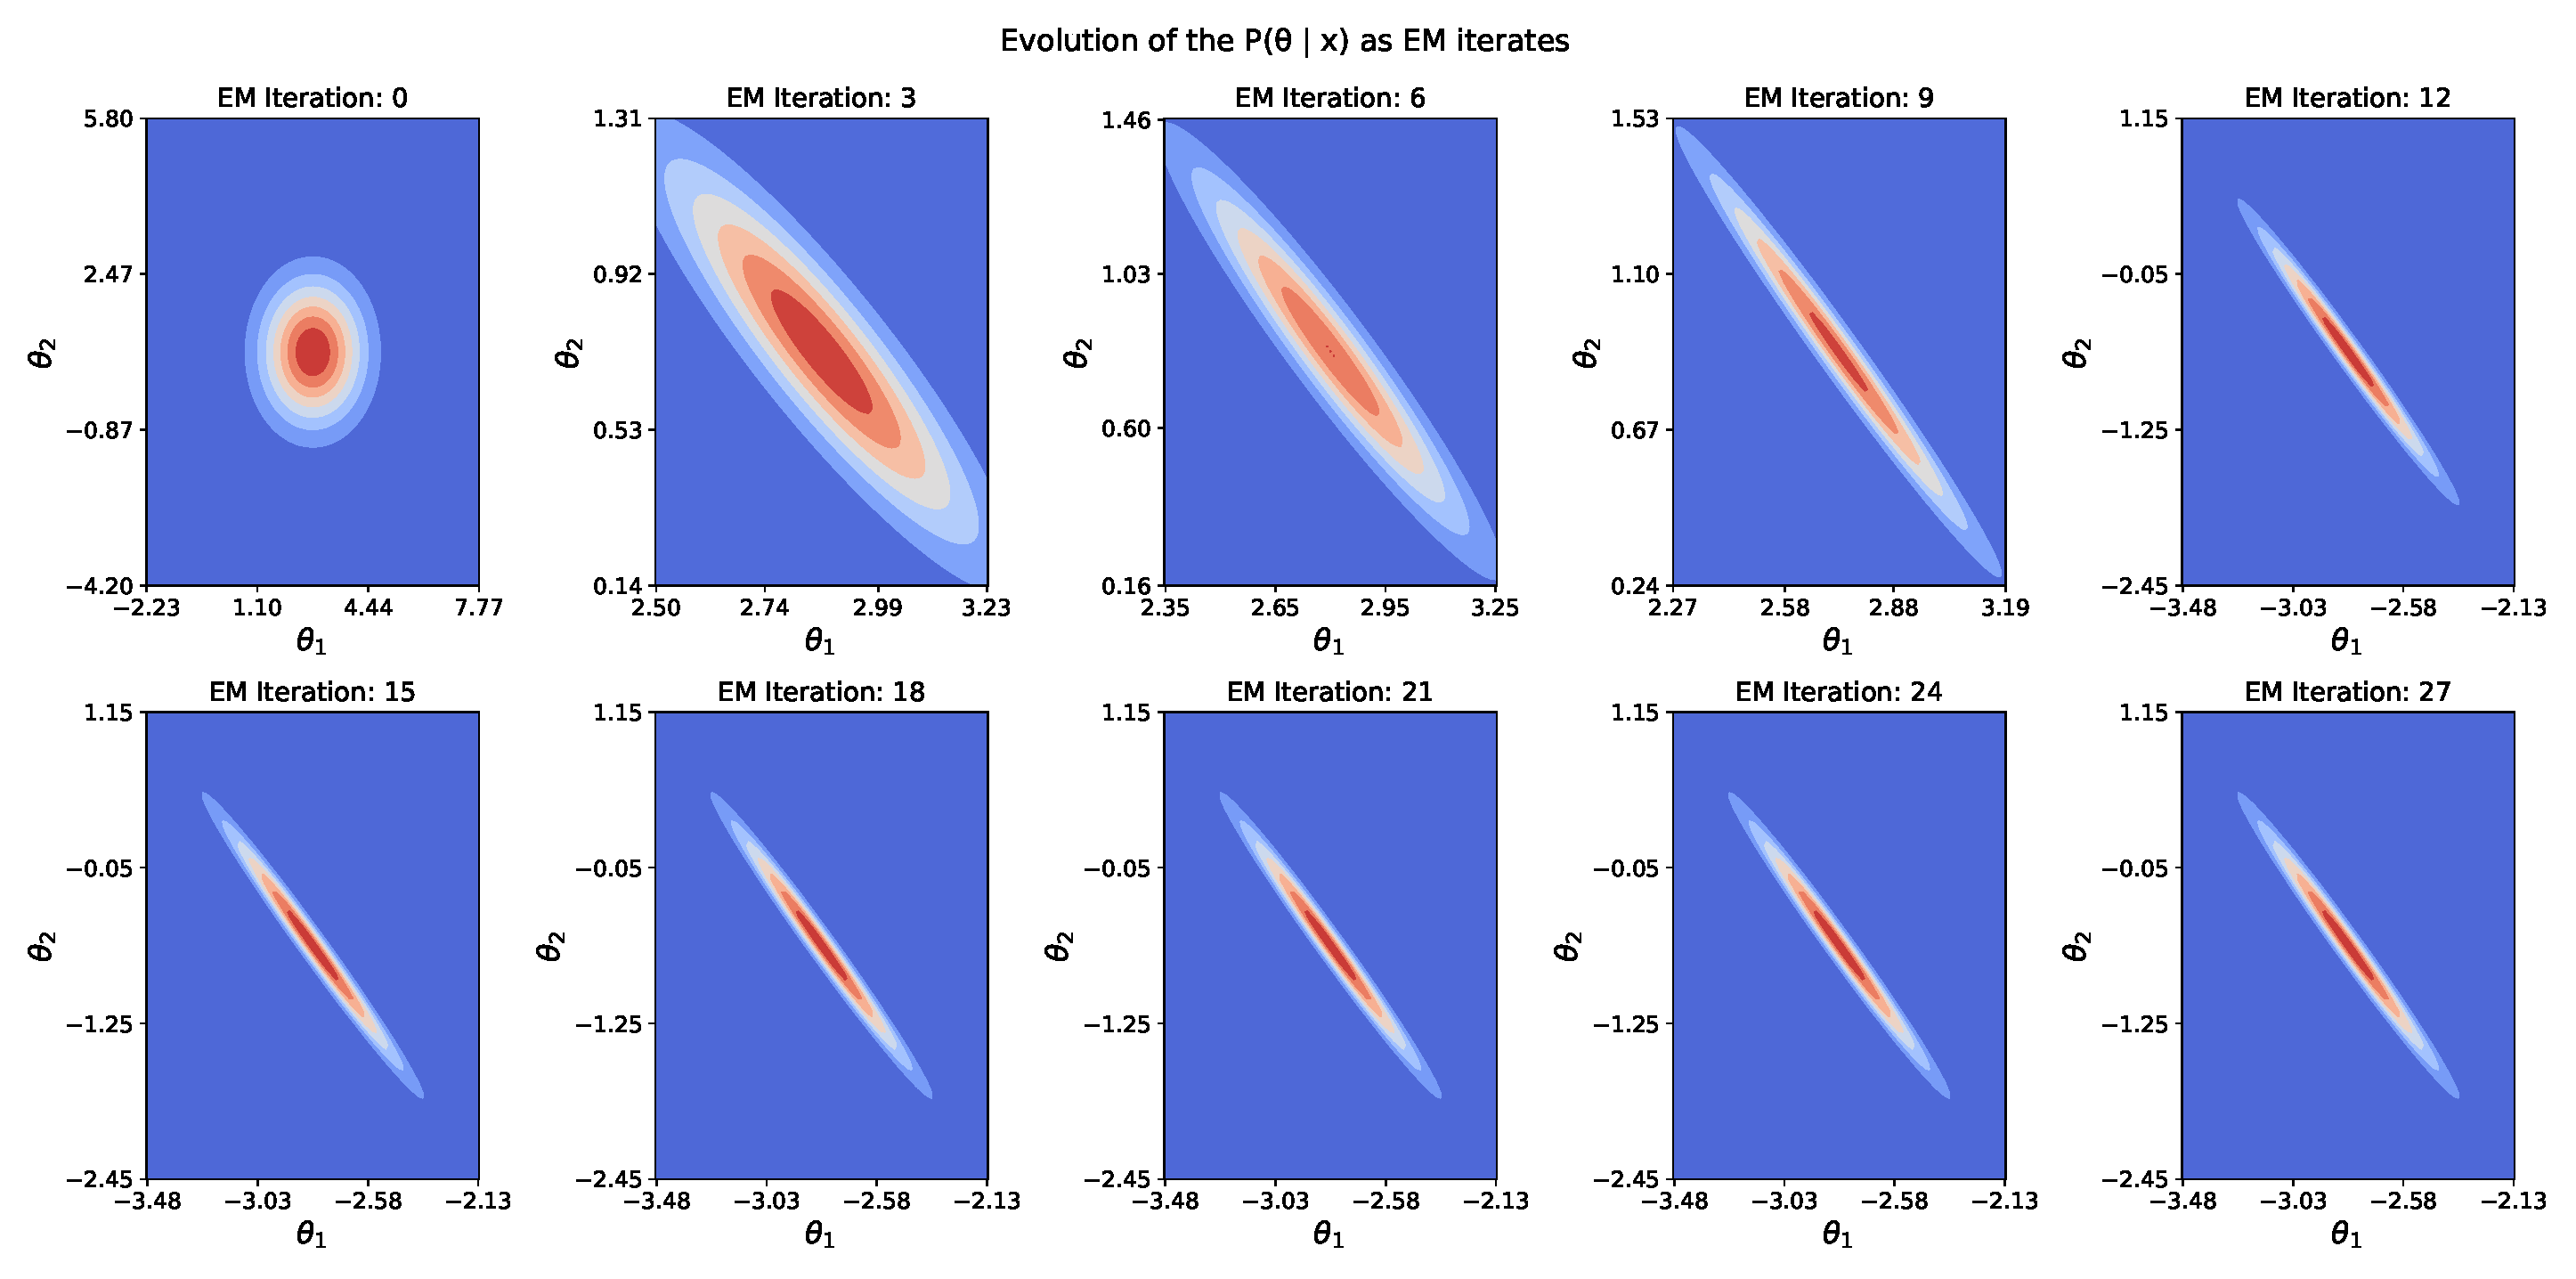
\includegraphics[width=\textwidth]{./figures/posterior_evolution.eps}
    \caption{(Progression: left-to-right then top-to-bottom) The evolution of
    the posterior distribution, $P(\theta \mid \mathrm{x})$, as the EM algorithm
    iterates. The end-effector location is $\mathrm{x} = \bmat{-1.5 & -0.4}$ as
    in Figure~\ref{fig:example_sol}. The posterior distribution $P(\theta \mid
    \mathrm{x})$ is marginalized over $\theta_3$ for visualization.}
    \label{fig:belief_evolution}
\end{figure}